\documentclass[11pt,a4paper]{article}
\usepackage[utf8]{inputenc}
\usepackage[T1]{fontenc}
\usepackage{lmodern}
\usepackage{microtype}
\usepackage[margin=0.7in,top=0.75in,bottom=0.75in,headheight=14pt]{geometry}
\usepackage{amsmath,amssymb,amsthm,mathtools}
\usepackage{xcolor}
\usepackage{fancyhdr}
\usepackage{lastpage}
\usepackage{tikz}
\usetikzlibrary{calc,arrows.meta}
\usepackage{tcolorbox}
\usepackage{hyperref}

% Explicit RGB Color Palette
\definecolor{primaryblue}{RGB}{20, 52, 94}
\definecolor{secondaryblue}{RGB}{37, 99, 168}
\definecolor{accentteal}{RGB}{13, 120, 117}
\definecolor{lightbg}{RGB}{246, 249, 254}
\definecolor{darkgray}{RGB}{45, 55, 72}
\definecolor{ansbg}{RGB}{240, 249, 245}
\definecolor{ansborder}{RGB}{38, 115, 87}
\definecolor{remarkbg}{RGB}{254, 249, 240}
\definecolor{remarkborder}{RGB}{204, 118, 33}
\definecolor{stepbg}{RGB}{248, 250, 252}
\definecolor{stepborder}{RGB}{203, 213, 225}

% Hyperref Setup
\hypersetup{
    colorlinks=true,
    linkcolor=secondaryblue,
    urlcolor=accentteal,
    citecolor=primaryblue,
    pdftitle={Analytical Geometry and Polar Conic Sections Solutions},
    pdfauthor={Advanced Mathematics Solutions}
}

% Header & Footer
\pagestyle{fancy}
\fancyhf{}
\fancyhead[L]{\small\color{darkgray}\textbf{Analytical Geometry \& Polar Coordinates}}
\fancyhead[R]{\small\color{darkgray}\textbf{Conic Sections \& Straight Lines}}
\fancyfoot[L]{\small\color{darkgray}\textit{Complete Step-by-Step Solutions}}
\fancyfoot[R]{\small\color{darkgray}Page \textbf{\thepage} of \textbf{\pageref{LastPage}}}
\renewcommand{\headrulewidth}{0.5pt}
\renewcommand{\footrulewidth}{0.3pt}

% Custom Styled Boxes
\newtcolorbox{problembox}[1]{
    colback=lightbg,
    colframe=primaryblue,
    arc=2mm,
    boxrule=1.1pt,
    width=\textwidth,
    fonttitle=\bfseries\large,
    coltitle=white,
    colbacktitle=primaryblue,
    title={#1},
    top=2mm, bottom=2mm, left=3mm, right=3mm
}

\newtcolorbox{ansbox}[1]{
    colback=ansbg,
    colframe=ansborder,
    arc=1.5mm,
    boxrule=1pt,
    width=\textwidth,
    fonttitle=\bfseries\color{white},
    coltitle=white,
    colbacktitle=ansborder,
    title={#1},
    top=2mm, bottom=2mm, left=3mm, right=3mm
}

\newtcolorbox{remarkbox}[1]{
    colback=remarkbg,
    colframe=remarkborder,
    arc=1.5mm,
    boxrule=0.8pt,
    width=\textwidth,
    fonttitle=\bfseries\small\color{white},
    coltitle=white,
    colbacktitle=remarkborder,
    title={#1},
    top=1.8mm, bottom=1.8mm, left=3mm, right=3mm
}

\newtcolorbox{stepbox}[1]{
    colback=stepbg,
    colframe=stepborder,
    arc=1.2mm,
    boxrule=0.5pt,
    width=\textwidth,
    fonttitle=\bfseries\small\color{primaryblue},
    coltitle=primaryblue,
    colbacktitle=stepbg,
    title={#1},
    top=1.3mm, bottom=1.3mm, left=2.5mm, right=2.5mm
}

\begin{document}

% ==============================================================================
% PAGE 1: PROBLEM 1 SETUP, DIAGRAM & HARMONIC MEAN FOR S
% ==============================================================================
\begin{center}
    {\LARGE\bfseries\color{primaryblue} Analytical Geometry \& Polar Coordinates}\\[1.5mm]
    {\large\color{secondaryblue}\textbf{Exhaustive Step-by-Step Solutions with Mathematical Proofs \& Diagrams}}\\[1.2mm]
    {\small\color{darkgray} Topics: Focal Chords of Conics, Harmonic Mean Property, Polar Lines, and Triangular Areas}
    \vspace{1.5mm}
    \hrule height 1pt
    \vspace{2mm}
\end{center}

\noindent
\begin{problembox}{Problem 1: Focal Chords of an Ellipse}
If $PSQ$ and $PS'R$ be two chords of an ellipse through the foci $S$ and $S'$ respectively, then prove that
\[
\frac{SP}{SQ} + \frac{S'P}{S'R}
\]
is independent of the position of $P$.
\end{problembox}

\subsubsection*{1. Geometric Setup and Mathematical Definitions}
Consider an ellipse centered at the origin with standard Cartesian equation $\dfrac{x^2}{a^2} + \dfrac{y^2}{b^2} = 1$ ($a > b > 0$):
\begin{itemize}\setlength{\itemsep}{1pt}
    \item \textbf{Parameters:} Semi-major axis $a$, semi-minor axis $b$, eccentricity $e = \sqrt{1 - b^2/a^2} < 1$.
    \item \textbf{Semi-latus Rectum:} $l = \dfrac{b^2}{a} = a(1 - e^2)$.
    \item \textbf{Foci:} $S(ae, 0)$ and $S'(-ae, 0)$ situated symmetrically on the major axis.
    \item \textbf{Focal Chords:} $PSQ$ is a chord through focus $S$, and $PS'R$ is a chord through focus $S'$.
\end{itemize}

\begin{center}
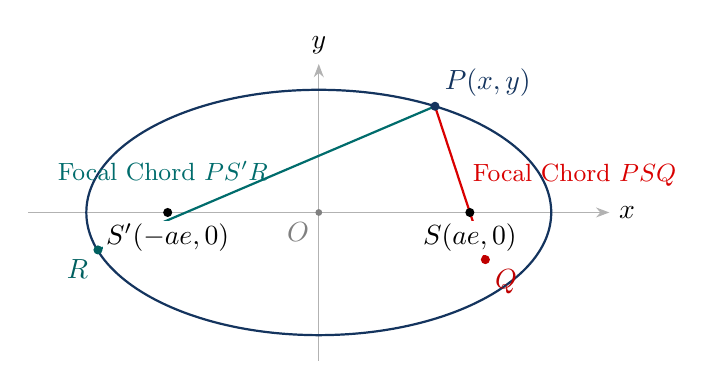
\begin{tikzpicture}[scale=0.82]
    % Axes
    \draw[->, >=Stealth, gray!60] (-4.5,0) -- (4.5,0) node[right, black] {$x$};
    \draw[->, >=Stealth, gray!60] (0,-2.3) -- (0,2.3) node[above, black] {$y$};
    
    % Ellipse: a = 3.6, b = 1.9
    \draw[thick, primaryblue] (0,0) ellipse (3.6cm and 1.9cm);
    
    % Foci
    \coordinate (S) at (2.34, 0);
    \coordinate (Sp) at (-2.34, 0);
    \coordinate (O) at (0, 0);
    
    % Point P on ellipse
    \coordinate (P) at (1.8, 1.645);
    \coordinate (Q) at (2.58, -0.73);
    \coordinate (R) at (-3.42, -0.58);
    
    % Draw Chords
    \draw[thick, red!85!black] (P) -- (Q);
    \draw[thick, teal!85!black] (P) -- (R);
    
    % Labels for Chords
    \node[red!85!black, right=2pt] at ($(P)!0.45!(Q)$) {\small Focal Chord $PSQ$};
    \node[teal!85!black, left=2pt] at ($(P)!0.45!(R)$) {\small Focal Chord $PS'R$};
    
    % Draw Points with background fill to avoid text clashes
    \fill[primaryblue] (P) circle (2pt) node[above right] {$P(x,y)$};
    \fill[red!75!black] (Q) circle (2pt) node[below right] {$Q$};
    \fill[teal!75!black] (R) circle (2pt) node[below left] {$R$};
    
    \fill[black] (S) circle (2pt);
    \node[below=3pt, fill=white, inner sep=1pt] at (S) {$S(ae,0)$};
    
    \fill[black] (Sp) circle (2pt);
    \node[below=3pt, fill=white, inner sep=1pt] at (Sp) {$S'(-ae,0)$};
    
    \fill[gray] (O) circle (1.5pt) node[below left] {$O$};
\end{tikzpicture}
\end{center}
\vspace{-3mm}

\subsubsection*{2. The Harmonic Mean Property of Focal Chords}
Take the focus $S$ as the pole and the major axis as the initial line. The polar equation of the ellipse is:
\[
\frac{l}{r} = 1 - e\cos\theta
\]
Let the vectorial angle of $P$ with respect to $S$ be $\alpha$. The radius vector is $SP = r_P$:
\[
\frac{l}{SP} = 1 - e\cos\alpha \implies \frac{1}{SP} = \frac{1 - e\cos\alpha}{l}
\]
Since $PSQ$ is a straight line through the pole $S$, point $Q$ has vectorial angle $\alpha + \pi$. Therefore:
\[
\frac{l}{SQ} = 1 - e\cos(\alpha + \pi) = 1 + e\cos\alpha \implies \frac{1}{SQ} = \frac{1 + e\cos\alpha}{l}
\]
Adding these two reciprocal equations yields the fundamental harmonic mean relation:
\begin{equation}\label{eq:harm_S}
\frac{1}{SP} + \frac{1}{SQ} = \frac{(1 - e\cos\alpha) + (1 + e\cos\alpha)}{l} = \frac{2}{l}
\end{equation}

\clearpage
% ==============================================================================
% PAGE 2: PROBLEM 1 RATIOS, INVARIANCE PROOF & CONCLUSION
% ==============================================================================
\subsubsection*{3. Expressing Segment Ratios and Establishing Invariance}

\paragraph{Segment Ratio for Chord $PSQ$ Through Focus $S$:}
Multiplying both sides of the harmonic mean relation \eqref{eq:harm_S} by $SP$:
\[
SP \left(\frac{1}{SP} + \frac{1}{SQ}\right) = SP \cdot \frac{2}{l} \implies 1 + \frac{SP}{SQ} = \frac{2 \cdot SP}{l} \implies \frac{SP}{SQ} = \frac{2 \cdot SP}{l} - 1
\]

\paragraph{Segment Ratio for Chord $PS'R$ Through Focus $S'$:}
Applying identical reasoning with the second focus $S'$ as the pole (the semi-latus rectum at $S'$ is also $l = b^2/a$):
\begin{equation}\label{eq:harm_Sp}
\frac{1}{S'P} + \frac{1}{S'R} = \frac{2}{l}
\end{equation}
Multiplying both sides of equation \eqref{eq:harm_Sp} by $S'P$:
\[
1 + \frac{S'P}{S'R} = \frac{2 \cdot S'P}{l} \implies \frac{S'P}{S'R} = \frac{2 \cdot S'P}{l} - 1
\]

\paragraph{Summing the Two Segment Ratios:}
Adding the two expressions:
\begin{align*}
\frac{SP}{SQ} + \frac{S'P}{S'R} &= \left(\frac{2 \cdot SP}{l} - 1\right) + \left(\frac{2 \cdot S'P}{l} - 1\right) = \frac{2(SP + S'P)}{l} - 2
\end{align*}
By the fundamental bifocal property of an ellipse, the sum of the focal distances from any point $P$ on the ellipse to the two foci is constant and identically equal to the length of the major axis $2a$:
\[
SP + S'P = 2a
\]
Substituting $SP + S'P = 2a$ into the summation formula:
\[
\frac{SP}{SQ} + \frac{S'P}{S'R} = \frac{2(2a)}{l} - 2 = \frac{4a}{l} - 2
\]
Substituting the value of the semi-latus rectum $l = \dfrac{b^2}{a} = a(1 - e^2)$:
\[
\frac{SP}{SQ} + \frac{S'P}{S'R} = \frac{4a}{\left(\dfrac{b^2}{a}\right)} - 2 = \frac{4a^2}{b^2} - 2 = \frac{4}{1 - e^2} - 2 = \frac{2(1 + e^2)}{1 - e^2}
\]

\vspace{5mm}
\noindent
\begin{ansbox}{Conclusion for Problem 1}
The evaluated expression:
\[
\mathbf{\frac{SP}{SQ} + \frac{S'P}{S'R} = \frac{2(1 + e^2)}{1 - e^2} = \frac{4a^2}{b^2} - 2}
\]
is a fixed constant determined exclusively by the ellipse parameters ($a, b, e$), and is \textbf{strictly independent of the position of point $P$}. \hfill $\blacksquare$
\end{ansbox}

\vspace{5mm}
\begin{remarkbox}{Physical and Geometric Significance}
Regardless of where $P$ traverses along the ellipse (at the ends of the major axis, ends of the minor axis, or any arbitrary location), as the chord through $S$ lengthens or shortens, the compensating chord through $S'$ adjusts in exact reciprocal proportion such that the combined ratio sum remains invariant.
\end{remarkbox}

\clearpage
% ==============================================================================
% PAGE 3: PROBLEM 2 SETUP, CONIC EQUATION & TANGENT SLOPES
% ==============================================================================
\noindent
\begin{problembox}{Problem 2: Angle Between Tangents at Extremities of a Focal Chord}
$PSP'$ is a focal chord of the conic. Prove that the angle between the tangents at $P$ and $P'$ is
\[
\tan^{-1}\left(\frac{2e\sin\alpha}{1 - e^2}\right)
\]
where $\alpha$ is the angle between the chord and the major axis.
\end{problembox}

\subsubsection*{1. Polar Equation of Conic and Extremities of the Chord}
Let the focus $S$ be the pole and the major axis (axis of the conic) be the initial line.
The polar equation of the conic is:
\[
\frac{l}{r} = 1 + e\cos\theta
\]
where $l$ is the semi-latus rectum and $e$ is the eccentricity.
The focal chord $PSP'$ passes through $S$ and makes an angle $\alpha$ with the initial line:
\begin{itemize}\setlength{\itemsep}{1pt}
    \item Point $P$ has vectorial angle $\theta_P = \alpha$.
    \item Point $P'$ lies on the opposite ray through the pole, with vectorial angle $\theta_{P'} = \alpha + \pi$.
\end{itemize}

\begin{center}
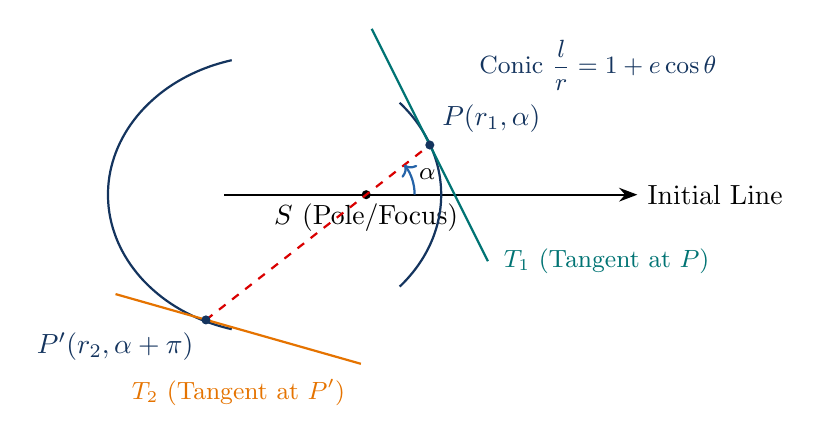
\begin{tikzpicture}[scale=0.82]
    % Initial line
    \draw[->, >=Stealth, thick] (-2.2,0) -- (4.2,0) node[right] {Initial Line};
    \coordinate (S) at (0,0);
    \fill (S) circle (2pt) node[below=2pt, fill=white, inner sep=1pt] {$S$ (Pole/Focus)};
    
    % Conic arc: r = l / (1 + e cos theta). Let l = 1.8, e = 0.55
    \draw[thick, primaryblue, domain=-70:70, samples=80] 
        plot ({1.8/(1 + 0.55*cos(\x))*cos(\x)}, {1.8/(1 + 0.55*cos(\x))*sin(\x)});
    \draw[thick, primaryblue, domain=135:225, samples=80] 
        plot ({1.8/(1 + 0.55*cos(\x))*cos(\x)}, {1.8/(1 + 0.55*cos(\x))*sin(\x)});
    \node[primaryblue, right] at (1.6, 2.0) {\small Conic $\dfrac{l}{r} = 1 + e\cos\theta$};
    
    % Focal chord at angle alpha = 38 deg
    \def\ang{38}
    \coordinate (P) at (\ang:1.25);
    \coordinate (Pp) at (\ang+180:3.15);
    
    % Draw Chord
    \draw[thick, dashed, red!85!black] (Pp) -- (P);
    
    % Angle alpha arc
    \draw[->, thick, secondaryblue] (0.75,0) arc (0:\ang:0.75);
    \node at (19:1.0) {\small $\alpha$};
    
    % Tangent lines
    \draw[thick, teal!90!black] ($(P) + (-0.9, 1.8)$) -- ($(P) + (0.9, -1.8)$) node[right=2pt] {\small $T_1$ (Tangent at $P$)};
    \draw[thick, orange!90!black] ($(Pp) + (-1.4, 0.4)$) -- ($(Pp) + (2.4, -0.68)$) node[below left=2pt] {\small $T_2$ (Tangent at $P'$)};
    
    % Points
    \fill[primaryblue] (P) circle (2pt) node[above right=1pt] {$P(r_1,\alpha)$};
    \fill[primaryblue] (Pp) circle (2pt) node[below left=1pt] {$P'(r_2,\alpha+\pi)$};
\end{tikzpicture}
\end{center}
\vspace{-3mm}

\subsubsection*{2. General Polar Tangent Equation and Slopes}
The equation of the tangent to the conic $\dfrac{l}{r} = 1 + e\cos\theta$ at a point with vectorial angle $\beta$ is:
\[
\frac{l}{r} = e\cos\theta + \cos(\theta - \beta) = (e + \cos\beta)\cos\theta + \sin\beta\sin\theta
\]
In Cartesian coordinates, where $x = r\cos\theta$ and $y = r\sin\theta$:
\begin{equation}\label{eq:tangent_cart}
(e + \cos\beta)x + (\sin\beta)y = l
\end{equation}
The slope of this tangent line is:
\[
m = -\frac{\text{coefficient of } x}{\text{coefficient of } y} = -\frac{e + \cos\beta}{\sin\beta}
\]
\paragraph{Slope of Tangent at $P$ ($\beta = \alpha$):}
\[
m_1 = -\frac{e + \cos\alpha}{\sin\alpha}
\]
\paragraph{Slope of Tangent at $P'$ ($\beta = \alpha + \pi$):}
Using $\cos(\alpha + \pi) = -\cos\alpha$ and $\sin(\alpha + \pi) = -\sin\alpha$:
\[
m_2 = -\frac{e + \cos(\alpha + \pi)}{\sin(\alpha + \pi)} = -\frac{e - \cos\alpha}{-\sin\alpha} = \frac{e - \cos\alpha}{\sin\alpha}
\]

\clearpage
% ==============================================================================
% PAGE 4: PROBLEM 2 EVALUATION & REMARKS
% ==============================================================================
\subsubsection*{3. Evaluation of the Angle Between the Two Tangents}
Let $\phi$ be the angle between the two tangents. By the standard slope formula:
\[
\tan\phi = \left| \frac{m_2 - m_1}{1 + m_1 m_2} \right|
\]

\begin{stepbox}{Step 3.1: Difference of Slopes $(m_2 - m_1)$}
\begin{align*}
m_2 - m_1 &= \frac{e - \cos\alpha}{\sin\alpha} - \left(-\frac{e + \cos\alpha}{\sin\alpha}\right) = \frac{(e - \cos\alpha) + (e + \cos\alpha)}{\sin\alpha} = \frac{2e}{\sin\alpha}
\end{align*}
\end{stepbox}

\begin{stepbox}{Step 3.2: Product of Slopes and Denominator $(1 + m_1 m_2)$}
\begin{align*}
m_1 m_2 &= \left(-\frac{e + \cos\alpha}{\sin\alpha}\right)\left(\frac{e - \cos\alpha}{\sin\alpha}\right) = -\frac{e^2 - \cos^2\alpha}{\sin^2\alpha}
\end{align*}
Adding 1 to both sides and using $\sin^2\alpha + \cos^2\alpha = 1$:
\[
1 + m_1 m_2 = 1 - \frac{e^2 - \cos^2\alpha}{\sin^2\alpha} = \frac{\sin^2\alpha - e^2 + \cos^2\alpha}{\sin^2\alpha} = \frac{1 - e^2}{\sin^2\alpha}
\]
\end{stepbox}

\begin{stepbox}{Step 3.3: Ratio $\tan\phi$}
\[
\tan\phi = \frac{m_2 - m_1}{1 + m_1 m_2} = \frac{\dfrac{2e}{\sin\alpha}}{\dfrac{1 - e^2}{\sin^2\alpha}} = \frac{2e}{\sin\alpha} \cdot \frac{\sin^2\alpha}{1 - e^2} = \frac{2e\sin\alpha}{1 - e^2}
\]
\end{stepbox}

\vspace{3mm}
\noindent
\begin{ansbox}{Conclusion for Problem 2}
Taking the inverse tangent, the angle $\phi$ between the tangents at $P$ and $P'$ is:
\[
\mathbf{\phi = \tan^{-1}\left(\frac{2e\sin\alpha}{1 - e^2}\right)}
\]
\hfill $\blacksquare$
\end{ansbox}

\vspace{3mm}
\begin{remarkbox}{Geometric Remarks \& Physical Insights}
\begin{enumerate}\setlength{\itemsep}{2pt}
    \item \textbf{Parabola ($e = 1$):} The denominator vanishes ($1 - e^2 = 0$), giving $\tan\phi \to \infty \implies \phi = 90^\circ$. Thus, the tangents at the extremities of any focal chord of a parabola are always mutually perpendicular and intersect on the directrix.
    \item \textbf{Latus Rectum ($\alpha = 90^\circ$):} Since $\sin 90^\circ = 1$, the angle between tangents at the ends of the latus rectum is $\tan^{-1}\left(\dfrac{2e}{1 - e^2}\right)$.
    \item \textbf{Intersection Point Locus:} The point of intersection of the tangents at the ends of a focal chord lies on the corresponding directrix $\dfrac{l}{r} = e\cos\theta$ for a parabola, and on the directrix line for general conics.
\end{enumerate}
\end{remarkbox}

\clearpage
% ==============================================================================
% PAGE 5: PROBLEM 3 SETUP, DIAGRAM & POLAR AREA EVALUATION
% ==============================================================================
\noindent
\begin{problembox}{Problem 3: Area of Triangle and Square in Polar Coordinates}
Find the area of the triangle whose vertices are $A(2, -30^\circ)$, $B(3, 120^\circ)$, and $C(1, 210^\circ)$. Also find the area of the square whose one side is $AC$.
\end{problembox}

\subsubsection*{1. Given Parameters and Polar Coordinate Diagram}
The vertices are given in polar coordinates $(r, \theta)$ as:
\[
A = (r_1, \theta_1) = (2, -30^\circ), \quad B = (r_2, \theta_2) = (3, 120^\circ), \quad C = (r_3, \theta_3) = (1, 210^\circ)
\]

\begin{center}
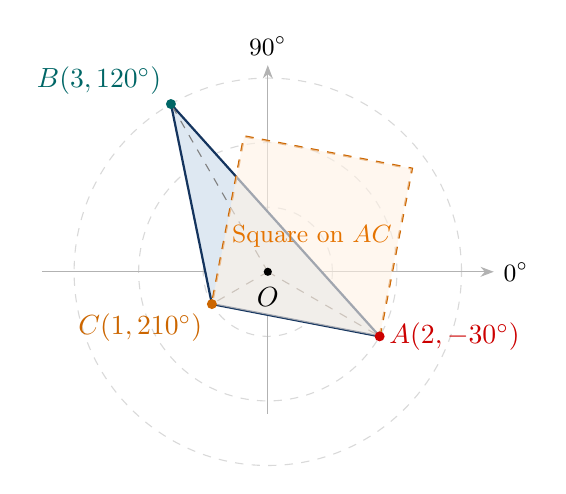
\begin{tikzpicture}[scale=0.82]
    % Concentric polar circles
    \draw[gray!30, dashed] (0,0) circle (1cm);
    \draw[gray!30, dashed] (0,0) circle (2cm);
    \draw[gray!30, dashed] (0,0) circle (3cm);
    
    % Polar axes
    \draw[->, >=Stealth, gray!60] (-3.5,0) -- (3.5,0) node[right, black] {\small $0^\circ$};
    \draw[->, >=Stealth, gray!60] (0,-2.2) -- (0,3.2) node[above, black] {\small $90^\circ$};
    
    % Polar Vertices
    \coordinate (A) at (-30:2);
    \coordinate (B) at (120:3);
    \coordinate (C) at (210:1);
    \coordinate (O) at (0,0);
    
    % Triangle ABC
    \fill[secondaryblue!15] (A) -- (B) -- (C) -- cycle;
    \draw[thick, primaryblue] (A) -- (B) -- (C) -- cycle;
    
    % Radii
    \draw[dashed, gray] (O) -- (A);
    \draw[dashed, gray] (O) -- (B);
    \draw[dashed, gray] (O) -- (C);
    
    % Square on AC
    \coordinate (V1) at ($(C)!1!90:(A)$);
    \coordinate (V2) at ($(A)!1!-90:(C)$);
    \draw[thick, dashed, orange!80!black] (A) -- (V2) -- (V1) -- (C);
    \fill[orange!10, opacity=0.6] (A) -- (V2) -- (V1) -- (C) -- cycle;
    \node[orange!90!black] at ($(V1)!0.5!(A)$) {\small Square on $AC$};
    
    % Nodes
    \fill[red!80!black] (A) circle (2.2pt) node[right] {$A(2, -30^\circ)$};
    \fill[teal!80!black] (B) circle (2.2pt) node[above left] {$B(3, 120^\circ)$};
    \fill[orange!80!black] (C) circle (2.2pt) node[below left] {$C(1, 210^\circ)$};
    \fill[black] (O) circle (1.8pt) node[below=2pt] {$O$};
\end{tikzpicture}
\end{center}
\vspace{-3mm}

\subsubsection*{2. Part 1: Area of Triangle $ABC$ (Direct Polar Formula)}
The area $\Delta$ of a triangle with vertices $(r_1, \theta_1)$, $(r_2, \theta_2)$, and $(r_3, \theta_3)$ in polar coordinates is:
\[
\Delta = \frac{1}{2} \left| r_1 r_2 \sin(\theta_2 - \theta_1) + r_2 r_3 \sin(\theta_3 - \theta_2) + r_3 r_1 \sin(\theta_1 - \theta_3) \right|
\]
Computing each term systematically:
\begin{enumerate}\setlength{\itemsep}{2pt}
    \item \textbf{Term 1:} $\theta_2 - \theta_1 = 120^\circ - (-30^\circ) = 150^\circ \implies r_1 r_2 \sin(150^\circ) = (2)(3)\left(\dfrac{1}{2}\right) = 3$
    \item \textbf{Term 2:} $\theta_3 - \theta_2 = 210^\circ - 120^\circ = 90^\circ \implies r_2 r_3 \sin(90^\circ) = (3)(1)(1) = 3$
    \item \textbf{Term 3:} $\theta_1 - \theta_3 = -30^\circ - 210^\circ = -240^\circ \implies \sin(-240^\circ) = \sin(60^\circ) = \dfrac{\sqrt{3}}{2} \implies r_3 r_1 \sin(-240^\circ) = (1)(2)\left(\dfrac{\sqrt{3}}{2}\right) = \sqrt{3}$
\end{enumerate}
Summing the three terms:
\[
\Sigma = 3 + 3 + \sqrt{3} = 6 + \sqrt{3} \implies \text{Area}(\triangle ABC) = \frac{6 + \sqrt{3}}{2} \approx 3.8660\text{ sq. units}
\]

\clearpage
% ==============================================================================
% PAGE 6: PROBLEM 3 CARTESIAN CHECK, SQUARE & CONCLUSION
% ==============================================================================
\paragraph{Cartesian Coordinate Verification for Triangle Area:}
Convert the vertices to Cartesian coordinates using $x = r\cos\theta$ and $y = r\sin\theta$:
\begin{itemize}\setlength{\itemsep}{1.5pt}
    \item $A(2, -30^\circ) \implies x_1 = 2\cos(-30^\circ) = \sqrt{3}, \quad y_1 = 2\sin(-30^\circ) = -1$
    \item $B(3, 120^\circ) \implies x_2 = 3\cos(120^\circ) = -\dfrac{3}{2}, \quad y_2 = 3\sin(120^\circ) = \dfrac{3\sqrt{3}}{2}$
    \item $C(1, 210^\circ) \implies x_3 = 1\cos(210^\circ) = -\dfrac{\sqrt{3}}{2}, \quad y_3 = 1\sin(210^\circ) = -\dfrac{1}{2}$
\end{itemize}
Using the standard Shoelace determinant formula:
\[
\Delta = \frac{1}{2}\left| x_1(y_2 - y_3) + x_2(y_3 - y_1) + x_3(y_1 - y_2) \right|
\]
\begin{align*}
x_1(y_2 - y_3) &= \sqrt{3}\left(\frac{3\sqrt{3} + 1}{2}\right) = \frac{9 + \sqrt{3}}{2}, \quad
x_2(y_3 - y_1) = -\frac{3}{2}\left(\frac{1}{2}\right) = -\frac{3}{4} \\
x_3(y_1 - y_2) &= -\frac{\sqrt{3}}{2}\left(-1 - \frac{3\sqrt{3}}{2}\right) = \frac{2\sqrt{3} + 9}{4}
\end{align*}
Summing the terms inside the absolute value:
\[
\frac{18 + 2\sqrt{3} - 3 + 2\sqrt{3} + 9}{4} = \frac{24 + 4\sqrt{3}}{4} = 6 + \sqrt{3} \implies \Delta = \frac{6 + \sqrt{3}}{2} \quad \checkmark
\]

\subsubsection*{3. Part 2: Area of the Square with Side $AC$}
The square of the side length $AC$ is calculated via the Law of Cosines in polar coordinates:
\[
AC^2 = r_1^2 + r_3^2 - 2 r_1 r_3 \cos(\theta_3 - \theta_1)
\]
Here $\theta_3 - \theta_1 = 210^\circ - (-30^\circ) = 240^\circ$. Since $\cos(240^\circ) = -\cos(60^\circ) = -\dfrac{1}{2}$:
\[
AC^2 = 2^2 + 1^2 - 2(2)(1)\left(-\frac{1}{2}\right) = 4 + 1 + 2 = 7
\]
\paragraph{Cartesian Distance Check:}
\[
AC^2 = (x_3 - x_1)^2 + (y_3 - y_1)^2 = \left(-\frac{3\sqrt{3}}{2}\right)^2 + \left(\frac{1}{2}\right)^2 = \frac{27}{4} + \frac{1}{4} = \frac{28}{4} = 7 \quad \checkmark
\]
Thus, the area of a square constructed on side $AC$ is:
\[
\text{Area of Square} = AC^2 = 7\text{ sq. units}
\]

\vspace{5mm}
\noindent
\begin{ansbox}{Final Result for Problem 3}
\begin{align*}
\textbf{Area of Triangle } ABC &= \mathbf{\frac{6 + \sqrt{3}}{2}} \text{ sq. units} \\[2mm]
\textbf{Area of Square on side } AC &= \mathbf{7} \text{ sq. units}
\end{align*}
Combined notation as recorded in original handwritten notes: $\mathbf{\left(\dfrac{6+\sqrt{3}}{2},\; 7\right)}$.
\end{ansbox}

\clearpage
% ==============================================================================
% PAGE 7: PROBLEM 4 COMPLETE SOLUTION
% ==============================================================================
\noindent
\begin{problembox}{Problem 4: Polar Equation of a Straight Line Through Two Points}
Find the polar equation of the straight line joining the two points $\left(1, \dfrac{\pi}{2}\right)$ and $(2, \pi)$.
\end{problembox}

\subsubsection*{1. Method 1: Using the Two-Point Polar Form}
The general equation of a straight line passing through points $P_1(r_1, \theta_1)$ and $P_2(r_2, \theta_2)$ is:
\begin{equation}\label{eq:polar_line_two_pt}
\frac{1}{r}\sin(\theta_2 - \theta_1) = \frac{1}{r_1}\sin(\theta_2 - \theta) + \frac{1}{r_2}\sin(\theta - \theta_1)
\end{equation}
The given points are $(r_1, \theta_1) = \left(1, \dfrac{\pi}{2}\right)$ and $(r_2, \theta_2) = (2, \pi)$:
\begin{itemize}\setlength{\itemsep}{1.5pt}
    \item $\theta_2 - \theta_1 = \pi - \dfrac{\pi}{2} = \dfrac{\pi}{2} \implies \sin(\theta_2 - \theta_1) = \sin\left(\frac{\pi}{2}\right) = 1$
    \item $\dfrac{1}{r_1}\sin(\theta_2 - \theta) = \dfrac{1}{1}\sin(\pi - \theta) = \sin\theta$
    \item $\dfrac{1}{r_2}\sin(\theta - \theta_1) = \dfrac{1}{2}\sin\left(\theta - \frac{\pi}{2}\right) = -\dfrac{1}{2}\cos\theta$
\end{itemize}
Substituting these into formula \eqref{eq:polar_line_two_pt}:
\[
\frac{1}{r}(1) = \sin\theta - \frac{1}{2}\cos\theta \implies \frac{2}{r} = 2\sin\theta - \cos\theta \iff 2 = r(2\sin\theta - \cos\theta)
\]

\begin{center}
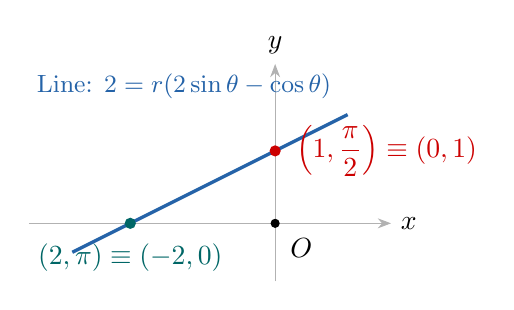
\begin{tikzpicture}[scale=0.92]
    % Axes
    \draw[->, >=Stealth, gray!60] (-3.4,0) -- (1.6,0) node[right, black] {$x$};
    \draw[->, >=Stealth, gray!60] (0,-0.8) -- (0,2.2) node[above, black] {$y$};
    \coordinate (O) at (0,0);
    \fill (O) circle (1.8pt) node[below right=2pt] {$O$};
    
    % Points: P1 = (0, 1), P2 = (-2, 0)
    \coordinate (P1) at (0,1);
    \coordinate (P2) at (-2,0);
    
    % Draw extended line through P2 and P1: slope = 1/2
    % Points on line: (-2.8, -0.4) to (1.0, 1.5)
    \draw[very thick, secondaryblue] (-2.8, -0.4) -- (1.0, 1.5) node[above left=2pt] {\small Line: $2 = r(2\sin\theta - \cos\theta)$};
    
    % Points and clean labels
    \fill[red!80!black] (P1) circle (2.2pt) node[right=4pt] {$\left(1, \dfrac{\pi}{2}\right) \equiv (0, 1)$};
    \fill[teal!80!black] (P2) circle (2.2pt) node[below=4pt] {$(2, \pi) \equiv (-2, 0)$};
\end{tikzpicture}
\end{center}
\vspace{-3mm}

\subsubsection*{2. Method 2: Verification via Cartesian Intercept Form}
Convert the given polar points to Cartesian coordinates $(x = r\cos\theta, y = r\sin\theta)$:
\begin{itemize}\setlength{\itemsep}{1.5pt}
    \item For $\left(1, \dfrac{\pi}{2}\right)$: $x_1 = 1\cos\left(\frac{\pi}{2}\right) = 0, \; y_1 = 1\sin\left(\frac{\pi}{2}\right) = 1 \implies (0, 1) \quad (\text{$y$-intercept } b = 1)$
    \item For $(2, \pi)$: $x_2 = 2\cos\pi = -2, \; y_2 = 2\sin\pi = 0 \implies (-2, 0) \quad (\text{$x$-intercept } a = -2)$
\end{itemize}
Using the two-intercept form of a straight line $\dfrac{x}{a} + \dfrac{y}{b} = 1$:
\[
\frac{x}{-2} + \frac{y}{1} = 1 \implies -x + 2y = 2 \implies 2y - x = 2
\]
Substituting the polar relations $x = r\cos\theta$ and $y = r\sin\theta$:
\[
2(r\sin\theta) - (r\cos\theta) = 2 \implies r(2\sin\theta - \cos\theta) = 2
\]

\vspace{3mm}
\noindent
\begin{ansbox}{Final Answer for Problem 4}
The required polar equation of the straight line is:
\[
\mathbf{2 = r(2\sin\theta - \cos\theta)} \quad \text{or} \quad \mathbf{\frac{2}{r} = 2\sin\theta - \cos\theta}
\]
\end{ansbox}

\clearpage
% ==============================================================================
% PAGE 8: PROBLEM 5 SETUP & GEOMETRIC PROOF
% ==============================================================================
\noindent
\begin{problembox}{Problem 5: Derivation of the General Polar Equation of a Straight Line}
Show that the polar equation of the straight line passing through the points $(r_1, \theta_1)$ and $(r_2, \theta_2)$ is
\[
\frac{1}{r}\sin(\theta_2 - \theta_1) = \frac{1}{r_1}\sin(\theta_2 - \theta) + \frac{1}{r_2}\sin(\theta - \theta_1)
\]
or in symmetric cyclic form:
\[
\frac{\sin(\theta_2 - \theta_1)}{r} + \frac{\sin(\theta - \theta_2)}{r_1} + \frac{\sin(\theta_1 - \theta)}{r_2} = 0
\]
\end{problembox}

\subsubsection*{1. Geometric Configuration}
Let $O$ be the pole (origin) and $OX$ the initial line. Let $A(r_1, \theta_1)$ and $B(r_2, \theta_2)$ be two given points on the straight line, with $\theta_2 > \theta_1$.
Let $P(r, \theta)$ be an arbitrary point on the straight line situated between $A$ and $B$, so that $\theta_1 \le \theta \le \theta_2$.

\begin{center}
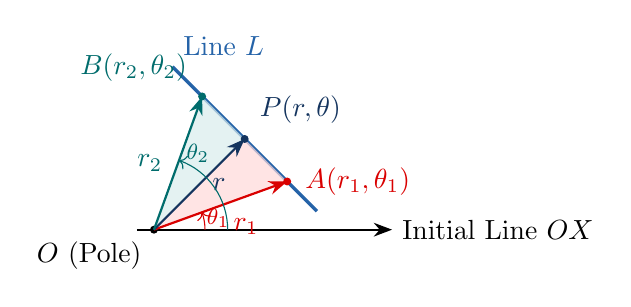
\begin{tikzpicture}[scale=0.72]
    % Pole and Initial Line
    \draw[->, >=Stealth, thick] (-0.3,0) -- (4.2,0) node[right] {Initial Line $OX$};
    \coordinate (O) at (0,0);
    \fill (O) circle (2pt) node[below left=1pt] {$O$ (Pole)};
    
    % Collinear points on line x + y = 3.2
    % A at theta1 = 20 deg, P at theta = 45 deg, B at theta2 = 70 deg
    \coordinate (A) at (2.35, 0.85);
    \coordinate (P) at (1.60, 1.60);
    \coordinate (B) at (0.85, 2.35);
    
    % Draw extended straight line L
    \draw[very thick, secondaryblue] ($(A)!-0.35!(B)$) -- ($(B)!-0.35!(A)$) node[above right] {Line $L$};
    
    % Shaded sub-triangles
    \fill[red!15, opacity=0.7] (O) -- (A) -- (P) -- cycle;
    \fill[teal!15, opacity=0.7] (O) -- (P) -- (B) -- cycle;
    
    % Vectors from pole
    \draw[thick, red!85!black, ->, >=Stealth] (O) -- (A) node[midway, below right=1pt] {$r_1$};
    \draw[thick, primaryblue, ->, >=Stealth] (O) -- (P) node[midway, right=1pt] {$r$};
    \draw[thick, teal!85!black, ->, >=Stealth] (O) -- (B) node[midway, left=2pt] {$r_2$};
    
    % Point nodes
    \fill[red!85!black] (A) circle (2pt) node[right=3pt] {$A(r_1, \theta_1)$};
    \fill[primaryblue] (P) circle (2pt) node[above right=2pt] {$P(r, \theta)$};
    \fill[teal!85!black] (B) circle (2pt) node[above left=2pt] {$B(r_2, \theta_2)$};
    
    % Angle arcs from initial line
    \draw[->, red!85!black] (0.9,0) arc (0:20:0.9);
    \node[red!85!black] at (10:1.15) {\footnotesize $\theta_1$};
    
    \draw[->, teal!85!black] (1.3,0) arc (0:70:1.3);
    \node[teal!85!black] at (60:1.55) {\footnotesize $\theta_2$};
\end{tikzpicture}
\end{center}
\vspace{-4mm}

\subsubsection*{2. Proof Method 1: By Addition of Triangular Areas (Geometric Proof)}
Since the points $A$, $P$, and $B$ are collinear, the segment $AB$ is partitioned into $AP$ and $PB$.
Consequently, the area of $\triangle OAB$ is the algebraic sum of the areas of the two sub-triangles $\triangle OAP$ and $\triangle OPB$:
\begin{equation}\label{eq:area_sum}
\text{Area}(\triangle OAB) = \text{Area}(\triangle OAP) + \text{Area}(\triangle OPB)
\end{equation}
Recall that the area of any triangle with two sides $p, q$ and included angle $\psi$ is given by $\dfrac{1}{2}pq\sin\psi$:
\begin{enumerate}\setlength{\itemsep}{1.5pt}
    \item \textbf{In $\triangle OAB$:} Sides $OA = r_1, OB = r_2$, included angle $\angle AOB = \theta_2 - \theta_1$:
    \[
    \text{Area}(\triangle OAB) = \frac{1}{2} r_1 r_2 \sin(\theta_2 - \theta_1)
    \]
    \item \textbf{In $\triangle OAP$:} Sides $OA = r_1, OP = r$, included angle $\angle AOP = \theta - \theta_1$:
    \[
    \text{Area}(\triangle OAP) = \frac{1}{2} r_1 r \sin(\theta - \theta_1)
    \]
    \item \textbf{In $\triangle OPB$:} Sides $OP = r, OB = r_2$, included angle $\angle POB = \theta_2 - \theta$:
    \[
    \text{Area}(\triangle OPB) = \frac{1}{2} r r_2 \sin(\theta_2 - \theta)
    \]
\end{enumerate}
Substituting these three expressions into equation \eqref{eq:area_sum}:
\[
\frac{1}{2} r_1 r_2 \sin(\theta_2 - \theta_1) = \frac{1}{2} r_1 r \sin(\theta - \theta_1) + \frac{1}{2} r r_2 \sin(\theta_2 - \theta)
\]
Divide both sides of the equation by $\dfrac{1}{2} r r_1 r_2$:
\[
\frac{r_1 r_2 \sin(\theta_2 - \theta_1)}{r r_1 r_2} = \frac{r r_2 \sin(\theta_2 - \theta)}{r r_1 r_2} + \frac{r_1 r \sin(\theta - \theta_1)}{r r_1 r_2}
\]
Simplifying each fraction:
\begin{equation}\label{eq:result_std}
\frac{1}{r}\sin(\theta_2 - \theta_1) = \frac{1}{r_1}\sin(\theta_2 - \theta) + \frac{1}{r_2}\sin(\theta - \theta_1)
\end{equation}
This completes the direct geometric proof. \hfill $\blacksquare$

\clearpage
% ==============================================================================
% PAGE 9: PROBLEM 5 ALGEBRAIC PROOF, CONNECTION & SYNTHESIS
% ==============================================================================
\subsubsection*{3. Proof Method 2: Via the General Linear Form and Determinants}
The general equation of a straight line in polar coordinates is:
\[
\frac{1}{r} = A\cos\theta + B\sin\theta
\]
where $A$ and $B$ are constants. Since points $A(r_1, \theta_1)$ and $B(r_2, \theta_2)$ lie on this line:
\begin{align}
A\cos\theta + B\sin\theta - \frac{1}{r} &= 0 \label{eq:det1}\\
A\cos\theta_1 + B\sin\theta_1 - \frac{1}{r_1} &= 0 \label{eq:det2}\\
A\cos\theta_2 + B\sin\theta_2 - \frac{1}{r_2} &= 0 \label{eq:det3}
\end{align}
For non-trivial constants $(A, B, -1)$, the determinant of coefficients must vanish:
\[
\begin{vmatrix}
\dfrac{1}{r} & \cos\theta & \sin\theta \\[2mm]
\dfrac{1}{r_1} & \cos\theta_1 & \sin\theta_1 \\[2mm]
\dfrac{1}{r_2} & \cos\theta_2 & \sin\theta_2
\end{vmatrix} = 0
\]
Expanding along the first column:
\[
\frac{1}{r}(\cos\theta_1\sin\theta_2 - \sin\theta_1\cos\theta_2) - \frac{1}{r_1}(\cos\theta\sin\theta_2 - \sin\theta\cos\theta_2) + \frac{1}{r_2}(\cos\theta\sin\theta_1 - \sin\theta\cos\theta_1) = 0
\]
Applying the sine difference formula $\sin(u - v) = \sin u\cos v - \cos u\sin v$:
\[
\frac{1}{r}\sin(\theta_2 - \theta_1) - \frac{1}{r_1}\sin(\theta_2 - \theta) + \frac{1}{r_2}\sin(\theta_1 - \theta) = 0
\]
Using $\sin(\theta_1 - \theta) = -\sin(\theta - \theta_1)$:
\[
\frac{1}{r}\sin(\theta_2 - \theta_1) = \frac{1}{r_1}\sin(\theta_2 - \theta) + \frac{1}{r_2}\sin(\theta - \theta_1)
\]
Rearranging to the cyclic symmetric form by using $\sin(\theta_2 - \theta) = -\sin(\theta - \theta_2)$:
\[
\frac{\sin(\theta_2 - \theta_1)}{r} + \frac{\sin(\theta - \theta_2)}{r_1} + \frac{\sin(\theta_1 - \theta)}{r_2} = 0
\]

\vspace{3mm}
\noindent
\begin{ansbox}{Summary of Equivalent Forms for Problem 5}
\begin{enumerate}\setlength{\itemsep}{2pt}
    \item \textbf{Standard Two-Point Polar Form:}
    \[
    \mathbf{\frac{1}{r}\sin(\theta_2 - \theta_1) = \frac{1}{r_1}\sin(\theta_2 - \theta) + \frac{1}{r_2}\sin(\theta - \theta_1)}
    \]
    \item \textbf{Cyclic Symmetric / Determinant Form:}
    \[
    \mathbf{\frac{\sin(\theta_2 - \theta_1)}{r} + \frac{\sin(\theta - \theta_2)}{r_1} + \frac{\sin(\theta_1 - \theta)}{r_2} = 0}
    \]
\end{enumerate}
\end{ansbox}

\vspace{3mm}
\begin{remarkbox}{Direct Deduction of Problem 4 from General Theorem 5}
Substituting $(r_1, \theta_1) = \left(1, \dfrac{\pi}{2}\right)$ and $(r_2, \theta_2) = (2, \pi)$ into Theorem 5:
\[
\frac{1}{r}\sin\left(\pi - \frac{\pi}{2}\right) = \frac{1}{1}\sin(\pi - \theta) + \frac{1}{2}\sin\left(\theta - \frac{\pi}{2}\right) \implies \frac{1}{r}(1) = \sin\theta - \frac{1}{2}\cos\theta \implies 2 = r(2\sin\theta - \cos\theta)
\]
which precisely recovers the exact solution to Problem 4.
\end{remarkbox}

\end{document}
